% !TeX root = ../../tesis.tex

% =============================================================================
%  SECCIÓN 3.3 — Indicadores de Análisis: Definición, Formulación y Aplicación
%  Archivo raíz — el contenido está subdividido en archivos 3-3-0 a 3-3-9
% =============================================================================

\section{Indicadores de Análisis: Definición, Formulación y Aplicación al
Caso de Estudio}
\label{sec:indicadores-formulas}

% !TeX root = ../../tesis.tex

% =============================================================================
%  3.3.0 — Introducción a los Indicadores de Análisis
% =============================================================================

El análisis computacional de la red de transporte público de la \cdmx{} y su
zona metropolitana se articula a través de ocho indicadores cuantitativos
organizados en cuatro fases de construcción progresiva. Esta jerarquía no es
arbitraria: cada indicador depende de los insumos producidos por los anteriores,
de modo que la arquitectura metodológica constituye en sí misma un modelo de
grafo que crece en complejidad desde el análisis espacial puro hasta las pruebas
de estrés topológico. A continuación se presenta cada uno de los indicadores con
su fundamento matemático, la fuente académica que lo sustenta, y un ejemplo
práctico calibrado con datos del área de estudio.

Los ocho indicadores están distribuidos entre los Objetivos Específicos 1 al 5
(§\ref{subsec:obj-especificos}): los indicadores de la Fase 1 ---$C$, $C_i$, $DI$ y $CF_h$--- alimentan los
Objetivos Específicos 2 y 4; el de la Fase 2 ---$W_{s,h}$--- refina el grafo
del Objetivo Específico 1; el Tiempo de Viaje
Promedio $T$ y la Centralidad de Intermediación $B(v)$ responden a los Objetivos
Específicos 2 y 3 respectivamente; y la Robustez Geométrica $\Delta E$ integra
los Objetivos Específicos 3 y 5 al cuantificar el efecto de la propuesta anillar
sobre la vulnerabilidad estructural de la red. La tabla de síntesis al final de
esta sección (§\ref{subsec:resumen-indicadores}) concentra estas
correspondencias de manera visual.

\bigskip
\noindent\textbf{Nota aclaratoria sobre el alcance de los indicadores.}
Todos los indicadores enumerados en este capítulo se definen en su fundamento
conceptual y matemático. No obstante, el indicador de
\textbf{Robustez Geométrica $\Delta E$} constituye una excepción en cuanto a su
demostración aplicada: por los tiempos del presente estudio y el enfoque de los
resultados esperados en las capas de código, $\Delta E$ no se implementa ni
valida empíricamente en los capítulos de desarrollo tecnológico. Su definición
formal se preserva aquí como marco teórico; la implementación computacional y la
validación sobre la red de la \zmvm{} se proponen como línea prioritaria de
investigación futura.

% !TeX root = ../../tesis.tex

% =============================================================================
\subsection*{Grupo 1: Indicadores Espaciales y de Cobertura}
% =============================================================================

% -----------------------------------------------------------------------
\subsection{Nivel de Cobertura de la Red de Transporte \texorpdfstring{$C$}{C}}
\label{subsec:indicador-cobertura}
% -----------------------------------------------------------------------

\textbf{Fuente principal:} \citet{fortin2016innovative}

\subsubsection{Definición y Fundamentación}

El nivel de cobertura es el indicador de entrada del modelo: el más
independiente de todos, pues su cálculo se realiza exclusivamente mediante
análisis espacial y no requiere que el grafo de la red esté completamente
interconectado. Mide la proporción del territorio urbano que queda dentro de una
distancia caminable de algún nodo de la red de transporte.

\citet{fortin2016innovative} explican en su sección de evaluación de
accesibilidad que los indicadores de cobertura más comunes se calculan trazando
áreas de influencia ---típicamente un \textit{buffer} de 500 metros o 400 metros
como radio de caminata promedio aceptable--- alrededor de cada parada de la red.
A partir de estas áreas, es posible identificar la proporción de individuos o de
empleos que quedan dentro de cierta distancia de la infraestructura de
transporte, lo que permite evaluar el nivel de accesibilidad en el territorio y
señalar con precisión los lugares donde deben ocurrir las mejoras.

\subsubsection{Fórmula}

\begin{equation}
    C = \frac{\text{Área Cubierta por Buffers}}{\text{Área Total de la Zona de Estudio}}
    \label{eq:cobertura}
\end{equation}

Donde:
\begin{itemize}
    \item $C$ = Nivel de Cobertura de la Red (adimensional, rango $[0, 1]$).
\item \textbf{Área Cubierta} = Unión de los polígonos de cobertura (isócronas o
    \textit{buffers} circulares) generados alrededor de cada parada de la red,
    medida en km².
\item \textbf{Área Total} = Superficie del polígono urbano delimitado de la zona
    de estudio, en km².
\end{itemize}

\begin{figure}[H]
    \centering
    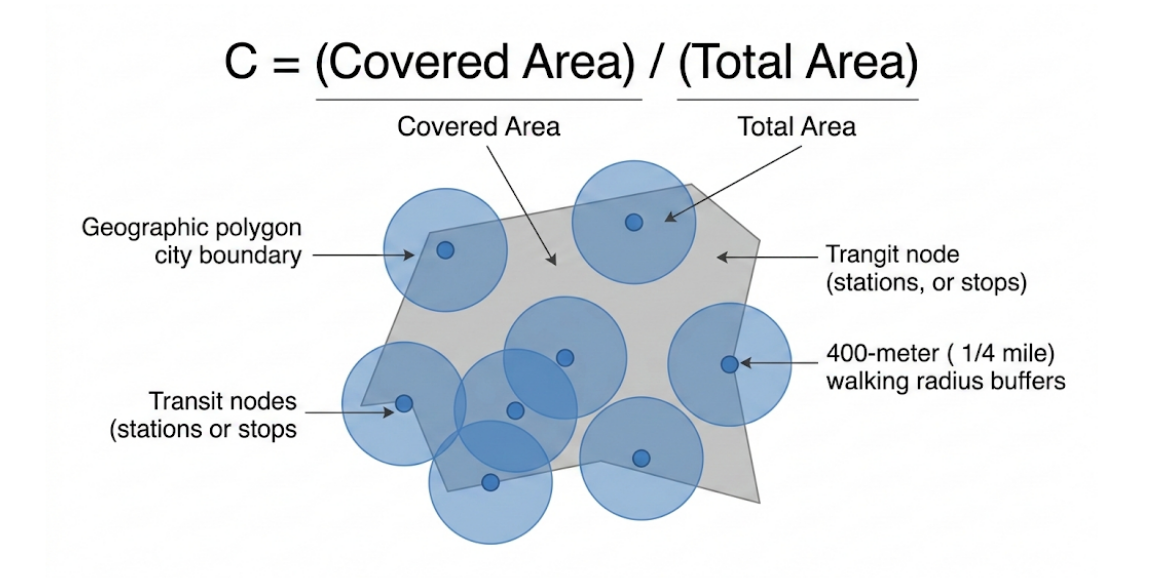
\includegraphics[width=0.80\textwidth]{Figures/Cap3/CoberturaTransporte.png}
    \caption[Diagrama del indicador de Cobertura $C$]{Esquema del cálculo del
indicador $C$: polígono de la zona de estudio (Área Total), nodos de transporte
    y círculos de radio 400\,m (Área Cubierta).}
    \label{fig:indicador-C}
    \fuentefigura{Elaboración propia con base en \citet{fortin2016innovative}.}
\end{figure}


\subsubsection{Consideraciones de Implementación}

Para una representación más precisa que la del \textit{buffer} circular
estático, se implementará el concepto de \termino{isócronas}: áreas de
influencia construidas a partir de la red vial real de OpenStreetMap, que
delimitan todos los puntos alcanzables caminando desde una parada en exactamente
15 minutos a la velocidad promedio peatonal (4.5 km/h en zonas densas). Las
isócronas producen polígonos irregulares que respetan barreras físicas como vías
rápidas, cuerpos de agua o pendientes pronunciadas, ofreciendo una medida de
cobertura sustancialmente más realista que un círculo uniforme.

El resultado de las isócronas se superpone al censo poblacional del INEGI para
calcular no solo el área cubierta, sino la \termino{población cubierta}: la
fracción de habitantes de la zona metropolitana que reside dentro del área de
influencia de alguna parada de la red.

\subsubsection{Ejemplo Práctico: \cdmx{} y Zona Metropolitana}

\textbf{Datos de entrada:} Coordenadas georreferenciadas de todas las paradas de
la red (Metro, Metrobús, RTP, Trolebús, Cablebús, Mexibús) en formato
\geojson{} ; polígono del área urbana de la \zmvm{} $\approx 7{,}866$\,km²; capa
de manzanas del INEGI con datos de población del Censo 2020.


\begin{table}[H]
    \centering
    \caption{Estimaciones del indicador $C$ por escenario de red.}
    \label{tab:cobertura-escenarios}
    \begin{tabularx}{\textwidth}{X r r}
        \toprule
        \textbf{Escenario} & \textbf{Área Cubierta} & \textbf{Cobertura $C$} \\
        \midrule
        Red masiva actual (solo Metro + Metrobús + Cablebús)
            & $\approx 450$\,km² & $C \approx 0.06$ \\
        Red completa actual (incluyendo RTP y concesionados)
            & $\approx 2{,}800$\,km² & $C \approx 0.36$ \\
        Red con propuesta del Anillo Periférico (+60 estaciones)
            & $\approx 3{,}150$\,km² & $C \approx 0.40$ \\
        \bottomrule
    \end{tabularx}
\end{table}

La implementación computacional de referencia para este indicador se encuentra
en el \autoref{anx:indicadores-implementacion} (§\ref{anx:impl-cobertura}).

Este indicador da cumplimiento al Objetivo Específico 4 (§
\ref{subsec:obj-especificos}): la cobertura $C$ medida por cuadrante geográfico
y por sistema es la métrica primaria para delimitar las zonas periféricas con
mayor déficit de acceso estructurado, que son el punto de partida para evaluar
la pertinencia del escenario hipotético anillar.

% !TeX root = ../../tesis.tex

% -----------------------------------------------------------------------
\subsection{Nivel de Alimentación Capilar --- Fuerza Nodal \texorpdfstring{($C_i$)}{(Ci)}}
\label{subsec:alimentacion-capilar}
% -----------------------------------------------------------------------

\textbf{Fuente principal:} \citet{lee2008}

\subsubsection{Definición y Fundamentación}

Una vez que las estaciones están georreferenciadas y las aristas de la red están
conectadas, el siguiente paso es identificar el rol funcional de cada nodo en la
jerarquía del sistema. \citet{lee2008}, en su análisis estadístico de la red de
metro de Seúl, establecen que cada estación puede caracterizarse por dos
propiedades complementarias: su \termino{grado} ($k$), definido como el número
de conexiones (aristas) que entran o salen del nodo, y su \termino{fuerza}
($s$), definida como la suma de los pesos (flujos de pasajeros) de todos los
enlaces conectados a esa estación.

Los autores demuestran que la distribución de la fuerza de los nodos en la red
de metro de Seúl sigue un comportamiento log-normal con un pico característico,
lo que indica que la mayoría de las estaciones atienden un volumen similar de
pasajeros, pero un pequeño número de nodos ---los grandes concentradores o
\textit{hubs}--- acumula flujos desproporcionadamente elevados. Este patrón es
directamente relevante para la red de la \cdmx{}, donde los macro-CETRAMs
(Pantitlán, Indios Verdes, Cuatro Caminos, Taxqueña) operan como \textit{hubs}
nodales que concentran la articulación entre las redes capilares de superficie y
las arterias masivas.

\subsubsection{Fórmula}

\begin{equation}
    C_i = \sum_{j \in S} A_{ij} \cdot \peso{i}{j}
    \label{eq:fuerza-nodal}
\end{equation}

Donde:
\begin{itemize}
    \item $C_i$ = Nivel de Alimentación Capilar (Fuerza Nodal) de la estación
    masiva $i$.
    \item $S$ = Subconjunto de rutas pertenecientes exclusivamente a la red de
    superficie (RTP, microbús, trolebús, concesionados).
\item $A_{ij}$ = Elemento de la matriz de adyacencia: 1 si la ruta de superficie
    $j$ conecta con la estación masiva $i$, 0 en caso contrario.
\item $\peso{i}{j}$ = Peso de la conexión: capacidad de pasajeros por hora o
flujo
    real medido de la ruta $j$ en la estación $i$.
\end{itemize}


\citet{lee2008} establecen que el peso $\peso{i}{j}$ de un enlace representa el
flujo de pasajeros que transita por él, y que la fuerza $s_i$ de una estación
corresponde al número de pasajeros que llegan y parten de ella. En el modelo
propuesto, $\peso{i}{j}$ se inicializa con la capacidad operativa declarada de
cada ruta y se refinará en fases posteriores con el Coeficiente de Fricción
Vial.

\begin{figure}[H]
    \centering
    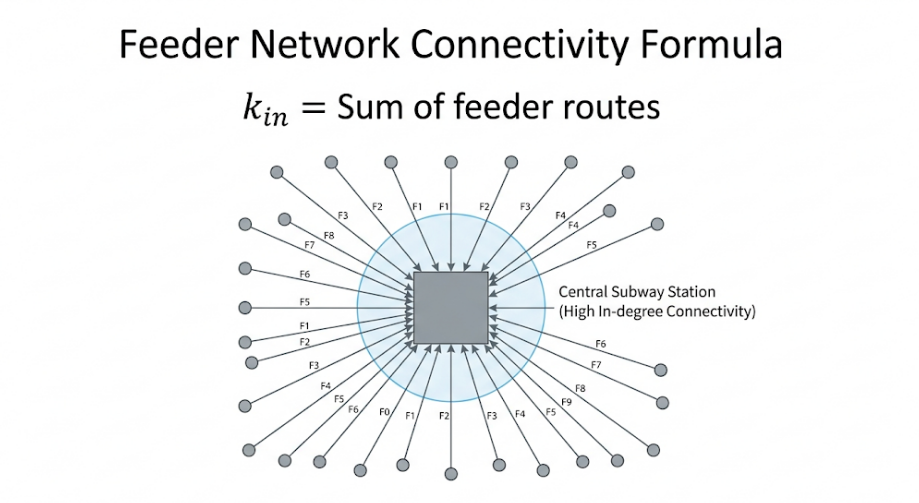
\includegraphics[width=0.70\textwidth]{Figures/Cap3/NiveldeAlimentacionCapilar.png}
    \caption[Diagrama del indicador de Alimentación Capilar $C_i$]{Esquema de
    fuerza nodal: rutas de superficie $F_1 \ldots F_n$ convergiendo en una
    estación masiva de alta conectividad de entrada.}
    \label{fig:indicador-Ci}
    \fuentefigura{Elaboración propia con base en \citet{lee2008}.}
 \end{figure}


\subsubsection{Ejemplo Práctico: \cdmx{} y Zona Metropolitana}

\begin{table}[H]
    \centering
    \caption{Estimaciones del indicador $C_i$ en nodos representativos.}
    \label{tab:capilar-nodos}
    \begin{tabularx}{\textwidth}{X r r}
        \toprule
        \textbf{Estación masiva} &
        \textbf{$k_{in}$ (rutas capilares)} &
        \textbf{$C_i$ estimado (pax/h)} \\
        \midrule
        Pantitlán (Hub CETRAM)          & $\approx 120$ rutas & Alto \\
        Indios Verdes (CETRAM)          & $\approx 90$ rutas  & Alto \\
        Nodo Norte propuesto (Periférico) & $\approx 40$ rutas (est.) & Medio-alto \\
        \bottomrule
    \end{tabularx}
\end{table}

La implementación computacional de referencia para este indicador se encuentra
en el \autoref{anx:indicadores-implementacion} (§\ref{anx:impl-capilar}).

La fuerza nodal $C_i$ complementa al indicador $C$ en la consecución del
Objetivo Específico 4 (§\ref{subsec:obj-especificos}): mientras $C$ mide el
alcance territorial de la red, $C_i$ cuantifica la intensidad de la articulación
capilar en cada nodo masivo, identificando cuáles de ellos concentran mayor
presión de demanda y constituyen, por tanto, los candidatos prioritarios para la
ampliación de la red con corredores perimetrales.

% !TeX root = ../../tesis.tex

% =============================================================================
\subsection*{Grupo 2: Indicadores de Eficiencia (Tiempo y Forma)}
% =============================================================================

% -----------------------------------------------------------------------
\subsection{Índice de Ruta Directa --- \texorpdfstring{\textit{Detour Factor} ($DI$)}{Detour Factor (DI)}}
\label{subsec:ruta-directa}
% -----------------------------------------------------------------------

\textbf{Fuente principal:} \citet{fortin2016innovative}

\subsubsection{Definición y Fundamentación}

El Índice de Ruta Directa cuantifica qué tan eficiente es la topología de la red
en términos geométricos puros: mide cuánto se alarga un viaje al estar obligado
a seguir la infraestructura real de la red en lugar de desplazarse en línea
recta entre origen y destino. \citet{fortin2016innovative} proponen este
indicador como parte de su método orientado a grafos para caracterizar
sistemáticamente redes de transporte a partir de datos \gtfs{}, donde el
análisis de la topología implica calcular los caminos mínimos entre pares de
nodos y derivar indicadores de desempeño.

Es importante precisar una limitación inherente: el $DI$ no incorpora los pesos
ponderados de las aristas (tiempos reales, frecuencias, factores de congestión),
sino únicamente la ubicación geométrica de los nodos. Es, por tanto, un
indicador de la \termino{eficiencia estructural} de la red ---independiente de
sus condiciones operativas--- y resulta especialmente útil para evaluar el
trazado de nuevas rutas o comparar configuraciones alternativas antes de
incorporar la dinámica de tráfico.

\subsubsection{Fórmula}

\begin{equation}
    DI = \frac{d_{\text{red}}(i,\, j)}{d_{\text{euclidiana}}(i,\, j)}
    \label{eq:detour-factor}
\end{equation}

Donde:
\begin{itemize}
    \item $DI$ = Índice de Ruta Directa (adimensional, siempre $DI \geq 1.0$).
\item $d_{\text{red}}(i, j)$ = Distancia del camino mínimo entre los nodos $i$
    y $j$ medida a lo largo de las aristas del grafo, en km.
    \item $d_{\text{euclidiana}}(i, j)$ = Distancia en línea recta (distancia
    \textit{haversine} para coordenadas geográficas) entre los nodos $i$ y $j$,
    en km.
\end{itemize}

Un valor $DI = 1.0$ representa eficiencia geométrica perfecta (el trayecto en
red coincide con la línea recta). Valores $DI \gg 1.0$ indican que la topología
fuerza a los usuarios a rodeos significativos respecto al desplazamiento ideal.

\begin{figure}[H]
    \centering
    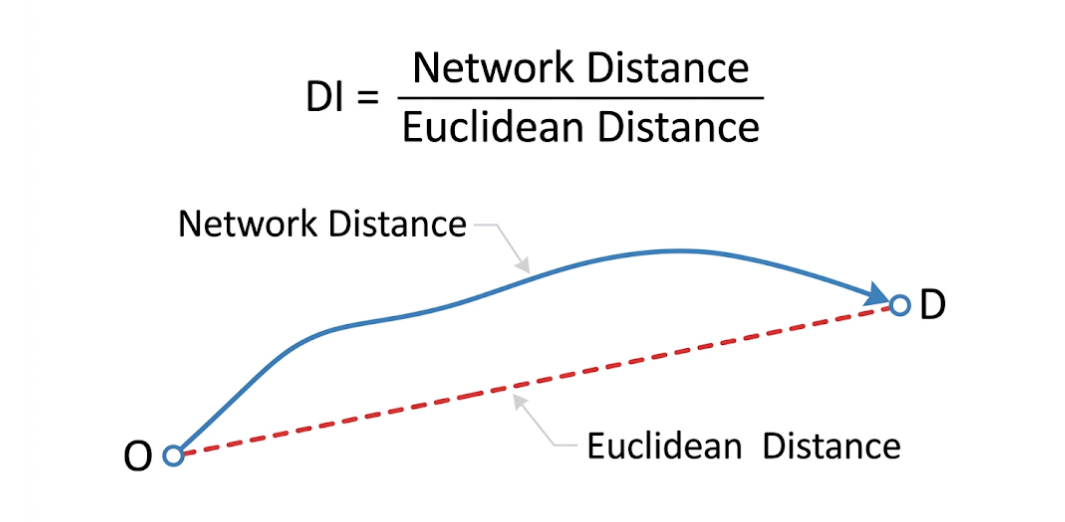
\includegraphics[width=0.65\textwidth]{Figures/Cap3/DistanciaEuclidiana.png}
    \caption[Diagrama del \textit{Detour Factor} $DI$]{Comparación entre la
    distancia en red (arco curvado) y la distancia euclidiana (línea punteada)
    entre origen O y destino D.}
    \label{fig:indicador-DI}
    \fuentefigura{Elaboración propia con base en \citet{fortin2016innovative}.}
\end{figure}

\subsubsection{Ejemplo Práctico: \cdmx{} y Zona Metropolitana}

\begin{table}[H]
    \centering
    \caption{Comparativa del indicador $DI$ antes y después del Anillo Periférico.}
    \label{tab:detour-factor}
    \begin{tabularx}{\textwidth}{X r r r r r}
        \toprule
        \textbf{Par O--D} &
        $d_{\text{eucl.}}$ &
        $d_{\text{red}}$ actual &
        $DI$ actual &
        $d_{\text{red}}$ con Anillo &
        $DI$ con Anillo \\
        \midrule
        Xochimilco $\to$ Santa Fe    & 15\,km & 28\,km & 1.87 & 18\,km & 1.20 \\
        Perisur $\to$ Naucalpan      & 18\,km & 42\,km & 2.33 & 26\,km & 1.44 \\
        Iztapalapa $\to$ Tlalnepantla & 22\,km & 55\,km & 2.50 & 30\,km & 1.36 \\
        \bottomrule
    \end{tabularx}
\end{table}

La implementación computacional de referencia para este indicador se encuentra
en el \autoref{anx:indicadores-implementacion} (§\ref{anx:impl-detour}).

El indicador $DI$ contribuye tanto al Objetivo Específico 2 ---en su papel de
métrica del diagnóstico topológico actual de la red--- como al Objetivo
Específico 5 (§\ref{subsec:obj-especificos}): la reducción del $DI$ entre pares
origen-destino del Tercer y Cuarto Contorno es uno de los efectos directamente
esperables y cuantificables de la incorporación del corredor anillar al grafo de
la \zmvm{}.

% !TeX root = ../../tesis.tex

% -----------------------------------------------------------------------
\subsection{Tiempo de Viaje Promedio \texorpdfstring{($T$)}{(T)}}
\label{subsec:tiempo-viaje}
% -----------------------------------------------------------------------

\textbf{Fuente principal:} \citet{aldous2019optimal}

\subsubsection{Definición y Fundamentación}

El Tiempo de Viaje Promedio es la métrica de desempeño global del sistema y el
criterio de optimización central del modelo. \citet{aldous2019optimal} plantean
que el criterio de optimalidad en el diseño de redes de transporte consiste en
minimizar el tiempo promedio de viaje entre pares de puntos elegidos
independientemente según su distribución en el territorio.

De manera particularmente relevante para la hipótesis central de este trabajo,
\citet{aldous2019optimal} demuestran analíticamente que, a medida que la
longitud total de la red aumenta, ocurre una transición brusca en un valor
crítico $L_c$ en el que aparece un bucle o anillo en la topología óptima de la
red. Esto implica que, para redes de transporte a escala metropolitana, la
incorporación de un corredor perimetral ---como el Anillo Periférico
propuesto--- no solo es viable, sino que constituye la forma
\textit{óptima esperada} de expansión de la red una vez superado cierto umbral
de longitud total. Este resultado teórico provee el sustento matemático directo
para la hipótesis de investigación.

\subsubsection{Fórmula}

\begin{equation}
    T = \frac{1}{N \cdot (N-1)} \sum_{i \neq j} t_{ij}
    \label{eq:tiempo-promedio}
\end{equation}

Donde:
\begin{itemize}
    \item $T$ = Tiempo de Viaje Promedio global de la red, en minutos.
    \item $N$ = Número total de nodos (estaciones y paradas) del grafo.
    \item $t_{ij}$ = Tiempo mínimo de viaje desde el nodo $i$ hasta el nodo $j$,
    calculado mediante el algoritmo de \dijkstra{} sobre el grafo ponderado,
    en minutos. Incluye tiempo en vehículo + tiempo de caminata + tiempo de
    espera en andén + penalización por transbordo.
\end{itemize}

El indicador $T$ se calculará en dos escenarios: la red metropolitana actual y
la red con la incorporación del Anillo Periférico. La diferencia
$\Delta T = T_{\text{actual}} - T_{\text{propuesto}}$ constituye la medida
cuantitativa principal de la viabilidad de la propuesta.

\begin{figure}[H]
    \centering
    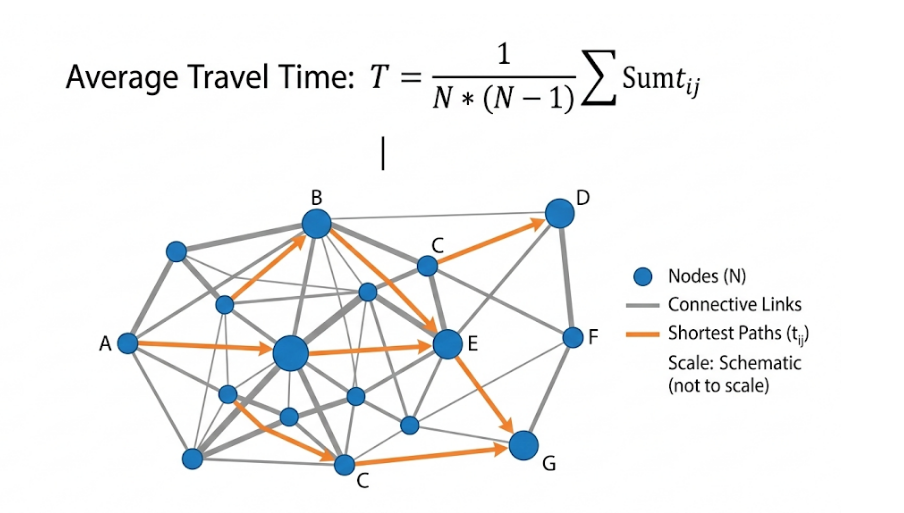
\includegraphics[width=0.72\textwidth]{Figures/Cap3/TiempoViajePromedio.png}
    \caption[Diagrama del indicador de Tiempo de Viaje Promedio $T$]{Red con
    nodos $N$, aristas grises (enlaces conectores) y caminos mínimos
    $t_{ij}$ (caminos más cortos) resaltados.}
    \label{fig:indicador-T}
    \fuentefigura{Elaboración propia con base en \citet{aldous2019optimal}.}
\end{figure}


\subsubsection{Ejemplo Práctico: \cdmx{} y Zona Metropolitana}

\begin{table}[H]
    \centering
    \caption{Estimaciones del indicador $T$ por escenario.}
    \label{tab:tiempo-promedio}
    \begin{tabularx}{\textwidth}{X r}
        \toprule
        \textbf{Escenario} & \textbf{$T$ estimado} \\
        \midrule
        Red radial actual (sin anillo) & $\approx 85$ minutos \\
        Red con propuesta del Anillo Periférico & $\approx 65$ minutos \\
        Reducción $\Delta T$ & $\approx 20$ min ($-24\%$) \\
        \bottomrule
    \end{tabularx}
\end{table}

La implementación computacional de referencia para este indicador se encuentra
en el \autoref{anx:indicadores-implementacion} (§\ref{anx:impl-tiempo}). La
proyección de paradas geográficas a nodos del grafo previa al cálculo de
$t_{ij}$ se describe en §\ref{subsubsec:snapping}.

El indicador $T$ es el criterio de optimización central de la investigación,
referenciado explícitamente en los Objetivos Específicos 2 y 5 (§
\ref{subsec:obj-especificos}). La diferencia
$\Delta T = T_{\text{actual}} - T_{\text{propuesto}}$ es la cifra que cuantifica
el beneficio global del escenario hipotético anillar; el resultado teórico de
\citet{aldous2019optimal} sobre la transición brusca en $L_c$ provee el sustento
matemático de por qué ese $\Delta T$ debe ser positivo para una red
metropolitana del tamaño de la \zmvm{}.

% !TeX root = ../../tesis.tex

% -----------------------------------------------------------------------
\subsection{Penalización por Transferencia \texorpdfstring{($W_{s,h}$)}{(Ws,h)}}
\label{subsec:penalizacion-transferencia}
% -----------------------------------------------------------------------

\textbf{Fuentes principales:} \citet{allauca2023}; \citet{aldous2019optimal}

\subsubsection{Definición y Fundamentación}

La penalización por transferencia es el costo temporal adicional en el que un
usuario incurre al cambiar de una línea o modo de transporte a otro durante su
viaje. Su correcta modelación es fundamental para que el grafo multimodal
refleje la experiencia real del usuario: un algoritmo de \dijkstra{} que no
penalice los transbordos subestimará sistemáticamente los tiempos de viaje en
rutas que requieren múltiples cambios de línea, induciendo al modelo a preferir
rutas con transbordos frecuentes que en la práctica resultan más lentas o
incómodas.

\citet{allauca2023} justifica la incorporación de pesos compuestos en las
aristas del grafo dirigido valorado como mecanismo para modelar correctamente el
costo total de cada ruta. La teoría de grafos provee algoritmos exactos de
caminos mínimos ---específicamente el algoritmo de \dijkstra{} y el algoritmo de
\floyd{}--- para determinar la ruta óptima entre cada par de nodos una vez que
los pesos de las aristas reflejan todos los componentes del costo de viaje.

\subsubsection{Fórmulas}

Se presentan dos variantes complementarias:

\medskip
\noindent\textbf{Variante 1 --- Penalización Estática (simplificada):}

\begin{equation}
    \text{Peso total} = T_{\text{viaje}} + \left(N_{\text{transbordos}}
    \times P_{\text{constante}}\right)
    \label{eq:penalizacion-estatica}
\end{equation}

Donde $P_{\text{constante}}$ es un castigo fijo de tiempo por cada transbordo
(valor de referencia: 12 minutos).

\medskip
\noindent\textbf{Variante 2 --- Penalización Dinámica (por arista de transferencia):}

\begin{equation}
    W_{s,h} = T_{\text{walk}}(s,\, h) + T_{\text{wait}}(s,\, h)
    \label{eq:penalizacion-dinamica}
\end{equation}

Donde:
\begin{itemize}
\item $W_{s,h}$ = Peso total de la arista artificial de transferencia entre la
    parada $s$ y el andén de la línea $h$, en minutos.
\item $T_{\text{walk}}(s, h)$ = Tiempo de caminata entre la parada de descenso
    y el andén de abordaje, en minutos.
    \item $T_{\text{wait}}(s, h)$ = Tiempo de espera promedio en el andén de la
    línea $h$, calculado como la mitad del intervalo de paso (\textit{headway})
    promedio de la línea.
\end{itemize}


\begin{figure}[H]
    \centering
    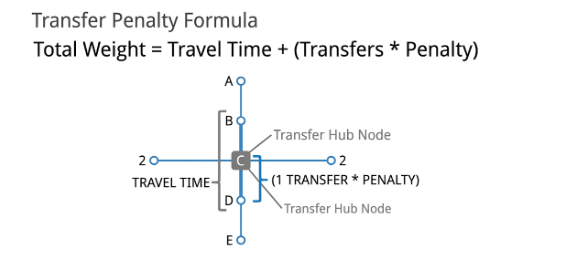
\includegraphics[width=0.68\textwidth]{Figures/Cap3/PenalizacionTransferencia.png}
    \caption[Diagrama del indicador de Penalización por Transferencia $W_{s,h}$]{
Nodo de transferencia con la descomposición del peso total en sus componentes
    de tiempo de caminata y espera.}
    \label{fig:indicador-W}
    \fuentefigura{Elaboración propia con base en \citet{allauca2023}.}
\end{figure}


\subsubsection{Nota Metodológica sobre Fuentes de Datos}

El uso de horarios \gtfs{} estáticos para estimar $T_{\text{wait}}$ introduce un
sesgo conocido: los datos estandarizados representan únicamente horarios
planificados, no tiempos reales de operación. \citet{fortin2016innovative}
reconocen esta limitación y señalan que los horarios inscritos pueden ser
incorrectos debido a la congestión o a errores de codificación. Para mitigar
este sesgo, la variante dinámica de la penalización se calibrará mediante
peticiones automatizadas a la \textit{Google Maps Directions API} (modo
\texttt{transit}, con variación del parámetro \texttt{departure\_time}), que
utiliza datos de \textit{crowdsourcing} (GPS de teléfonos móviles) para devolver
tiempos de espera y caminata ajustados a condiciones históricas reales en
distintos cortes horarios.

\subsubsection{Proyección Geográfica al Grafo: el Concepto de \termino{Snapping}}
\label{subsubsec:snapping}

Los indicadores $T$ y $W_{s,h}$ se calculan sobre nodos del grafo, pero los
datos de entrada ---paradas GTFS y puntos de transbordo--- son coordenadas
geográficas que rara vez coinciden con exactitud con algún nodo de la red OSM.
El \termino{snapping} resuelve esa discrepancia: para cada punto $p$ con
coordenadas $(lat, lon)$, la operación identifica el nodo más cercano
$v^* \in \mathcal{V}$ del grafo y lo adopta como representante:

\begin{equation}
    v^* = \arg\min_{v \in \mathcal{V}}\; d\!\left(p,\, v\right)
    \label{eq:snapping}
\end{equation}

donde $d(p, v)$ es la distancia haversine entre el punto geográfico y el nodo
del grafo. Sin este paso, el cálculo de $T_{\text{walk}}(s, h)$ sería
indefinido: el algoritmo no sabría desde qué nodo computar la ruta peatonal
hacia el andén de destino. El snapping constituye así el puente entre la
representación matemática del grafo y la geografía urbana real de la red,
haciendo posible traducir coordenadas de campo en insumos del modelo
\citep{fortin2016innovative}.

\subsubsection{Ejemplo Práctico: \cdmx{} y Zona Metropolitana}

\textbf{Par de transferencia:} Pantitlán Línea 1 Metro $\to$ Pantitlán Línea 9
Metro.

\begin{table}[H]
    \centering
    \caption{Estimaciones del indicador $W_{s,h}$ en la transferencia Pantitlán L1--L9.}
    \label{tab:penalizacion}
    \begin{tabularx}{\textwidth}{X r r}
        \toprule
        \textbf{Componente} & \textbf{Valor estático} &
        \textbf{Valor dinámico (hora pico 8:00\,h)} \\
        \midrule
        $T_{\text{walk}}$ (caminata entre andenes) & 3 min & 5 min \\
        $T_{\text{wait}}$ (espera en andén L9) & 4.5 min & 7 min \\
        $W_{s,h}$ \textbf{total} & \textbf{7.5 min} & \textbf{12 min} \\
        \bottomrule
    \end{tabularx}
\end{table}

El modelado correcto de $W_{s,h}$ es condición necesaria para que el grafo
multimodal construido en el Objetivo Específico 1 (§
\ref{subsec:obj-especificos} ) refleje la experiencia real del usuario. Un
algoritmo que omita esta penalización subestimaría los tiempos de viaje en rutas
multimodales e invalidaría el diagnóstico del Objetivo Específico 2, donde la
comparación entre escenarios descansa sobre la fidelidad del modelo de costos.

% !TeX root = ../../tesis.tex

% -----------------------------------------------------------------------
\subsection{Coeficiente de Fricción Vial \texorpdfstring{($CF_h$)}{(CFh)}}
\label{subsec:friccion-vial}
% -----------------------------------------------------------------------

\textbf{Fuente principal:} \citet{fortin2016innovative}

\subsubsection{Definición y Fundamentación}

El Coeficiente de Fricción Vial es un multiplicador dinámico que corrige la
sobreestimación de eficiencia que ocurre cuando se asigna a las rutas de
transporte de superficie un tiempo de viaje ideal, sin considerar el efecto de
la congestión vehicular. \citet{fortin2016innovative} reconocen que los datos
estandarizados del \gtfs{} representan únicamente horarios planificados, y que
utilizar tiempos ajustados a las condiciones reales de tráfico devuelve
estimaciones sustancialmente más precisas al ejecutar el algoritmo de
\dijkstra{}.

Este indicador distingue dos categorías de modos con comportamientos
radicalmente distintos respecto a la congestión: los \termino{modos confinados}
(Metro, Cablebús, Suburbano, Tren Ligero), que circulan en infraestructura
segregada y mantienen un $CF = 1.0$ constante, y los
\termino{modos de tráfico mixto} (RTP, Trolebús, Metrobús en tramos compartidos,
microbuses concesionados), cuyo tiempo de viaje real se incrementa en función de
la hora del día y las condiciones de la vialidad.

\subsubsection{Fórmula}

\begin{equation}
    CF_h = \frac{T_{\text{real},h}}{T_{\text{ideal}}}
    \label{eq:friccion-vial}
\end{equation}

\begin{equation}
    T_{\text{real},h} = T_{\text{ideal}} \times CF_h
    \label{eq:tiempo-real}
\end{equation}

Donde:
\begin{itemize}
    \item $CF_h$ = Coeficiente de Fricción Vial en la franja horaria $h$
    (adimensional, $CF_h \geq 1.0$).
\item $T_{\text{real},h}$ = Tiempo de viaje observado en el tramo a la hora $h$,
    en minutos.
    \item $T_{\text{ideal}}$ = Tiempo de viaje en condiciones de flujo libre
    (referencia: 05:00\,h, sin congestión), en minutos.
\end{itemize}

\subsubsection{Ejemplo Práctico: \cdmx{} y Zona Metropolitana}

Los valores de $T_{\text{real},h}$ que permiten calcular $CF_h$ se obtienen del
\textbf{TomTom Traffic Index} \citep{tomtom2024}, base de datos histórica que
registra la velocidad promedio de cada corredor vial de la \cdmx{} por franja
horaria y día de la semana. Para cada arista de tráfico mixto del grafo, el
coeficiente se estima como el cociente entre el tiempo real medido a la hora $h$
y el tiempo de referencia en condiciones de flujo libre (05:00\,h).

\textbf{Tramo de referencia:} Ruta RTP, Insurgentes Norte (5\,km, tiempo en
flujo libre: 10 minutos).

\begin{table}[H]
    \centering
    \caption{Valores del coeficiente $CF_h$ por franja horaria.}
    \label{tab:friccion-vial}
    \begin{tabularx}{\textwidth}{X r r}
        \toprule
        \textbf{Franja horaria} & \textbf{$T_{\text{real}}$ observado} &
        \textbf{$CF_h$} \\
        \midrule
        05:00\,h (flujo libre)          & 10 min   & 1.00 (referencia) \\
        08:00\,h (pico máximo)          & 18.5 min & \textbf{1.85} \\
        15:00\,h (pico vespertino)      & 16 min   & 1.60 \\
        19:00\,h (pico nocturno)        & 17 min   & 1.70 \\
        Metro (cualquier hora)          & 10 min   & \textbf{1.00} (confinado) \\
        \bottomrule
    \end{tabularx}
\end{table}

El coeficiente $CF_h$ calibra las aristas de tráfico mixto del grafo construido
en el Objetivo Específico 1 (§\ref{subsec:obj-especificos}): sin esta
corrección, los datos \gtfs{} estáticos producirían un modelo que sobreestima la
eficiencia de los modos de superficie y subestima la brecha operativa entre los
modos confinados y los concesionados, distorsionando el diagnóstico de la red
actual que el Objetivo Específico 2 requiere.

% !TeX root = ../../tesis.tex

% =============================================================================
\subsection*{Grupo 3: Topología y Rigor Matemático}
% =============================================================================

% -----------------------------------------------------------------------
\subsection{Centralidad de Intermediación (\termino{Betweenness Centrality}) \texorpdfstring{($B(v)$)}{(B(v))}}
\label{subsec:centralidad-intermediacion}
% -----------------------------------------------------------------------

\textbf{Fuentes principales:} \citet{lee2008}; \citet{allauca2023}

\subsubsection{Definición y Fundamentación}

La Centralidad de Intermediación ---denominada en la literatura anglosajona
\termino{betweenness centrality}--- cuantifica la importancia de cada nodo de la
red en función de cuántas rutas óptimas de la ciudad lo utilizan como nodo de
paso. Un nodo con alta centralidad de intermediación es aquel que aparece con
mayor frecuencia en los caminos mínimos entre los distintos pares origen-destino
del sistema: su remoción o saturación produce el mayor impacto sobre los tiempos
de viaje globales.

\citet{allauca2023} señala que la representación de la red de transporte como un
grafo permite realizar un análisis de centralidad para evaluar la importancia de
los nodos (estaciones), lo que sirve fundamentalmente para identificar los nodos
críticos y las rutas más importantes del sistema. \citet{lee2008}, en su caso de
estudio del metro de Seúl, aplican este principio empíricamente, demostrando que
en un sistema metropolitano la distribución del grado nodal sigue una ley de
potencias, confirmando la naturaleza de red libre de escala del sistema y su
consecuente vulnerabilidad a ataques dirigidos.

\subsubsection{Fórmula}

\begin{equation}
    B(v) = \sum_{s \neq v \neq t} \frac{\sigma_{st}(v)}{\sigma_{st}}
    \label{eq:betweenness}
\end{equation}

Donde:
\begin{itemize}
\item $B(v)$ = Centralidad de Intermediación de la estación $v$ (adimensional,
    normalizada en $[0, 1]$).
    \item $\sigma_{st}$ = Número total de caminos mínimos desde la estación de
    origen $s$ hasta el destino $t$.
    \item $\sigma_{st}(v)$ = Número de esos caminos mínimos que pasan
    forzosamente por la estación $v$.
\end{itemize}

La versión ponderada del indicador, $B(v, w)$, utiliza el tiempo de viaje real
como métrica de costo en la búsqueda de caminos mínimos, de modo que los nodos
contabilizados son aquellos que aparecen en las rutas más rápidas, no
necesariamente las más cortas en distancia.


\begin{figure}[H]
    \centering
    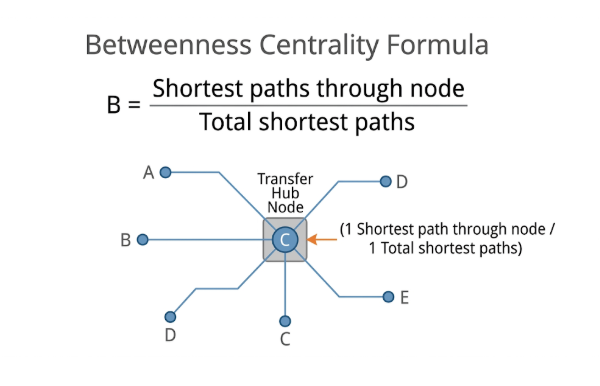
\includegraphics[width=0.62\textwidth]{Figures/Cap3/CentralidadItnermediacion.png}
    \caption[Diagrama de Centralidad de Intermediación $B(v)$]{Nodo de
    transferencia con alta centralidad: concentra el mayor número de caminos
    mínimos del sistema.}
    \label{fig:indicador-Bv}
    \fuentefigura{Elaboración propia con base en \citet{lee2008} y
    \citet{allauca2023}.}
\end{figure}


\subsubsection{Ejemplo Práctico: \cdmx{} y Zona Metropolitana}

\begin{table}[H]
    \centering
    \caption{Variación del indicador $B(v)$ antes y después del Anillo Periférico.}
    \label{tab:betweenness}
    \begin{tabularx}{\textwidth}{X r r r}
        \toprule
        \textbf{Nodo} & \textbf{$B(v)$ Red Actual} &
        \textbf{$B(v)$ con Anillo} & \textbf{Variación} \\
        \midrule
        Pantitlán               & $\approx 0.40$ & $\approx 0.22$ & $-45\%$ \\
        Pino Suárez             & $\approx 0.38$ & $\approx 0.20$ & $-47\%$ \\
        Tacubaya                & $\approx 0.35$ & $\approx 0.19$ & $-46\%$ \\
        Estaciones Anillo (prom.) & ---          & $\approx 0.18$ & $+\infty$ (nuevos) \\
        \bottomrule
    \end{tabularx}
\end{table}

La caída en la centralidad de intermediación de los nodos del centro de la
ciudad, combinada con el surgimiento de nuevos nodos de alta centralidad en el
Anillo Periférico, constituye la demostración algorítmica de que la propuesta
descongestiona el núcleo urbano y redistribuye los flujos hacia la periferia.

La implementación computacional de referencia para este indicador se encuentra
en el \autoref{anx:indicadores-implementacion} (§\ref{anx:impl-betweenness}).

La Centralidad de Intermediación es la métrica central del Objetivo Específico 3
(§\ref{subsec:obj-especificos}): identificar los nodos cuya pérdida
comprometería la conectividad global del sistema equivale a encontrar los nodos
que maximizan $B(v)$ en la red actual. Los valores de la tabla anterior
anticipan que Pantitlán, Pino Suárez y Tacubaya concentran desproporcionadamente
los flujos de la red radial, vulnerabilidad que el corredor anillar mitiga al
distribuir esa centralidad sobre nuevos nodos perimetrales.

% !TeX root = ../../tesis.tex

% -----------------------------------------------------------------------
\subsection{Robustez Geométrica --- Vulnerabilidad \texorpdfstring{($\Delta E$)}{(Delta E)}}
\label{subsec:robustez-geometrica}
% -----------------------------------------------------------------------

\textbf{Fuente principal:} \citet{lotero2014vulnerabilidad}

\subsubsection{Definición y Fundamentación}

La Robustez Geométrica es el indicador de mayor dependencia jerárquica del
modelo: para calcularlo, se requiere conocer previamente qué nodo destruir
---dado por el Indicador de Centralidad de Intermediación (
\autoref{subsec:centralidad-intermediacion})--- y medir el impacto de esa
destrucción sobre el desempeño global ---dado por el Indicador de Tiempo de
Viaje Promedio (\autoref{subsec:tiempo-viaje})---.

\citet{lotero2014vulnerabilidad} definen la vulnerabilidad operativamente como
la disminución de la eficiencia de la red después de un ataque o falla. La
metodología estándar para medir la robustez consiste en cuantificar el impacto
de la remoción de un componente de la red, ya sea de forma aleatoria
---simulando una falla fortuita como el cierre de una estación por inundación o
mantenimiento--- o de forma dirigida hacia los elementos más importantes,
simulando un ataque a un nodo crítico. Los autores señalan que las redes con
distribución libre de escala son robustas ante fallas aleatorias, pero altamente
vulnerables ante ataques dirigidos a sus nodos más conectados, resultado que es
la base teórica del experimento de fase final del presente trabajo.

\subsubsection{Fórmula}

\begin{equation}
    \Delta E = \frac{E_0 - E_f}{E_0}
    \label{eq:robustez}
\end{equation}

Donde:
\begin{itemize}
\item $\Delta E$ = Caída relativa de eficiencia de la red tras la remoción de un
    nodo o conjunto de nodos (adimensional, rango $[0, 1]$).
\item $E_0$ = Eficiencia global de la red en el estado completo, expresada como
    el inverso del Tiempo de Viaje Promedio:
    $E_0 = 1 / T_{\text{completa}}$.
\item $E_f$ = Eficiencia global de la red en el estado fallido (tras la remoción
    del nodo o nodos críticos):
    $E_f = 1 / T_{\text{fallida}}$.
\end{itemize}

Un valor $\Delta E \approx 0$ indica que la red es robusta: la pérdida del nodo
no afecta significativamente el desempeño global (existen rutas alternativas
eficientes). Un valor $\Delta E \to 1$ indica que la red es frágil: la pérdida
de ese nodo produce una degradación severa del servicio.


\begin{figure}[H]
    \centering
    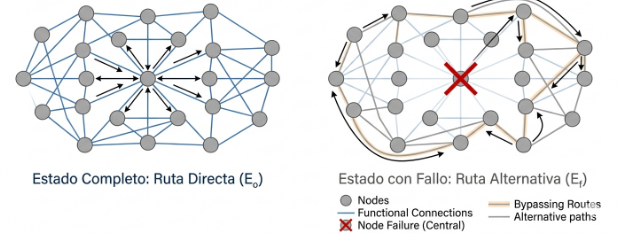
\includegraphics[width=0.80\textwidth]{Figures/Cap3/RobustezGeometrica.png}
    \caption[Diagrama del indicador de Robustez Geométrica $\Delta E$]{Estado
    completo con ruta directa ($E_0$) versus estado con fallo y rutas
    alternativas de desvío ($E_f$).}
    \label{fig:indicador-deltaE}
    \fuentefigura{Elaboración propia con base en \citet{lotero2014vulnerabilidad}.}
\end{figure}


\subsubsection{Ejemplo Práctico: \cdmx{} y Zona Metropolitana}

\textbf{Experimento:} Remoción del nodo ``Pantitlán'' (nodo de mayor $B(v)$ en
la red actual).

\begin{table}[H]
    \centering
    \caption{Impacto del indicador $\Delta E$ ante la remoción de Pantitlán.}
    \label{tab:robustez}
    \begin{tabularx}{\textwidth}{X r r r}
        \toprule
        \textbf{Condición} & \textbf{$T$ promedio} &
        \textbf{$E = 1/T$} & \textbf{$\Delta E$} \\
        \midrule
        Red actual completa ($E_0$)          & 85 min & 0.01176 & --- \\
        Red actual sin Pantitlán ($E_f$)     & 133 min & 0.00752 & $\mathbf{36\%}$ \\
        Red con Anillo completo ($E_0'$)     & 65 min & 0.01538 & --- \\
        Red con Anillo sin Pantitlán ($E_f'$) & 78 min & 0.01282 & $\mathbf{17\%}$ \\
        \bottomrule
    \end{tabularx}
\end{table}

La diferencia entre $\Delta E = 36\%$ (red radial sin anillo) y
$\Delta E = 17\% $ (red con anillo periférico) demuestra algorítmicamente que la
propuesta reduce la vulnerabilidad del sistema ante la pérdida del nodo más
crítico en casi un 53\%, dotando a la red metropolitana de redundancia
estructural.

La implementación computacional de referencia para este indicador se encuentra
en el \autoref{anx:indicadores-implementacion} (§\ref{anx:impl-robustez}).
Conforme a la nota aclaratoria de §\ref{sec:indicadores-formulas}, la validación
empírica de $\Delta E$ queda propuesta como línea de investigación futura.

El indicador $\Delta E$ articula los Objetivos Específicos 3 y 5 (§
\ref{subsec:obj-especificos}): la comparación de $\Delta E_{\text{actual}}$ con
$\Delta E_{\text{anillo}}$ ante la remoción de los nodos más críticos del
sistema demuestra si el corredor anillar propuesto reduce efectivamente la
fragilidad de la red, dotándola de rutas alternativas capaces de absorber la
demanda desplazada. Es, en este sentido, el indicador que cierra el argumento de
la investigación al ligar la hipótesis urbanística con la demostración
algorítmica.

% !TeX root = ../../tesis.tex

% =============================================================================
\subsection{Resumen de Indicadores y Fases de Construcción}
\label{subsec:resumen-indicadores}
% =============================================================================

La Tabla~\ref{tab:resumen-indicadores} concentra los ocho indicadores con su
símbolo, la fase metodológica correspondiente y las dependencias jerárquicas
entre ellos.

\begin{table}[H]
    \centering
    \caption{Resumen de los ocho indicadores de análisis y sus fases de
             construcción.}
    \label{tab:resumen-indicadores}
    \begin{tabularx}{\textwidth}{c >{\raggedright\arraybackslash}X c c >{\raggedright\arraybackslash}X}
        \toprule
        \textbf{\#} & \textbf{Indicador} & \textbf{Símbolo} &
        \textbf{Fase} & \textbf{Dependencias} \\
        \midrule
        1 & Nivel de Cobertura de la Red     & $C$          & 1 & Ninguna (espacial puro) \\
        2 & Nivel de Alimentación Capilar    & $C_i$        & 1 & Indicador 1 \\
        3 & Índice de Ruta Directa           & $DI$         & 1 & Indicadores 1--2 \\
        4 & Coeficiente de Fricción Vial     & $CF_h$       & 1 & Ninguna (datos históricos externos) \\
        5 & Penalización por Transferencia   & $W_{s,h}$    & 2 & Indicadores 1--4 \\
        6 & Tiempo de Viaje Promedio         & $T$          & 3 & Fases 1 y 2 completas \\
        7 & Centralidad de Intermediación (\termino{Betweenness Centrality}) & $B(v)$ & 3 & Indicadores 1--6 \\
        8 & Robustez Geométrica              & $\Delta E$   & 4 & Todos los anteriores \\
        \bottomrule
    \end{tabularx}
\end{table}

